% !TEX root = ../main.tex

\chapter{Literature review}

% ---- Section 2.1 ----
\section{Structural stability and the mechanics of non-linear materials}

\subsection{Column buckling and the normalised slenderness approach}

Perfect columns are idealised structural members that are perfectly straight and present linear elastic, perfectly plastic behaviour. The strength of such members is bounded by two limiting modes of failure: geometric instability and material yielding. The former is governed by the Euler critical buckling load, which for a pin-ended column is 
%
\begin{equation}
    N_{\mathrm{cr}} = \frac{\pi^2 E I}{L^2},
    \label{eq:euler}
\end{equation}
%
where $E$ is the Young's modulus, $I$ is the second moment of area and $L$ is the member length \parencite{timoshenko2009}. The latter is governed by the squash load $N_{\mathrm{y}} = A f_{\mathrm{y}}$, where $A$ is the cross-sectional area and $f_{\mathrm{y}}$ is the yield stress. These parameters define the normalised slenderness $\lambdabar$, which collapses the column's geometry, material and length into a single dimensionless parameter, while the ultimate load $N_{\mathrm{u}}$ is normalised against the squash load to give the strength-reduction factor $\chi$:
%
\begin{align}
    \lambdabar &= \sqrt{\frac{N_{\mathrm{y}}}{N_{\mathrm{cr}}}}, &
    \chi &= \frac{N_{\mathrm{u}}}{N_{\mathrm{y}}}.
    \label{eq:slenderness-chi}
\end{align}
%
As illustrated in \cref{fig:chi-lambdabar-baseline}, the theoretical maximum strength of a perfect column forms a sharp $\chi$--$\lambdabar$ baseline: a pure squashing plateau ($\chi = 1$) for stocky columns and an elastic Euler hyperbola ($\chi = \lambdabar^{-2}$) for slender columns, the two regimes meeting at $\lambdabar = 1$ \parencite{trahair2008}.

\begin{figure}[htbp]
  \centering
  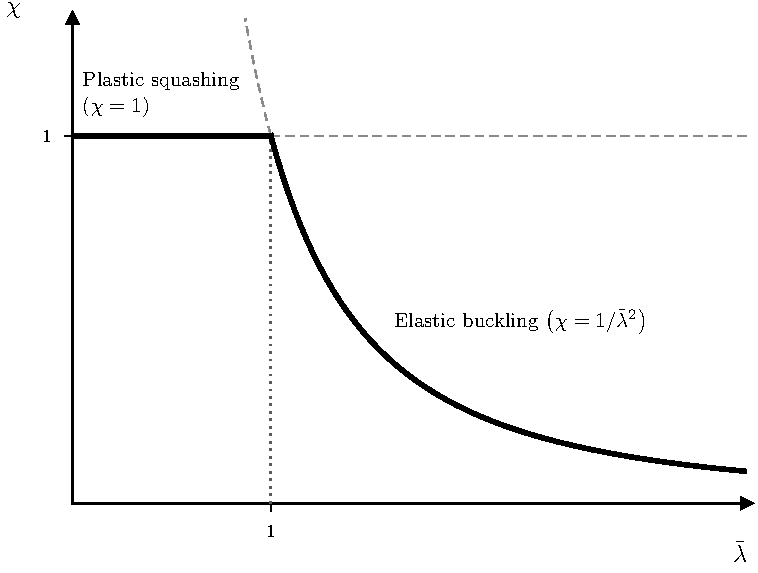
\includegraphics[width=0.8\textwidth]{figures/chi-lambdabar-baseline.pdf}
  \caption[Idealised column strength baseline ($\chi$--$\lambdabar$)]{%
    Non-dimensional buckling reduction factor $\chi$ against member slenderness
    $\lambdabar$ for a geometrically perfect column of elastic--perfectly plastic
    material. The strength baseline is the lower envelope of two regimes: a plastic
    squashing plateau ($\chi = 1$) governing stocky members and the elastic Euler
    hyperbola ($\chi = \lambdabar^{-2}$) governing slender members, the two
    intersecting at $\lambdabar = 1$.}
  \label{fig:chi-lambdabar-baseline}
\end{figure}

\subsection{The Ramberg–Osgood constituitive law for non-linear materials}

\section{Design philosophies for non-linear material buckling}
\subsection{Empirical buckling curves and the Eurocode 3 approach}
\subsection{The tangent-modulus approach}

\section{The Köllner–Gardner–Wadee (2023) energy formulation and its open question}
\subsection{A closed-form solution for Ramberg–Osgood struts}
\subsection{The correction factor $\beta$}